\documentclass{standalone}
\usepackage{tikz}
\usetikzlibrary{circuits.ee.IEC}

\begin{document}
    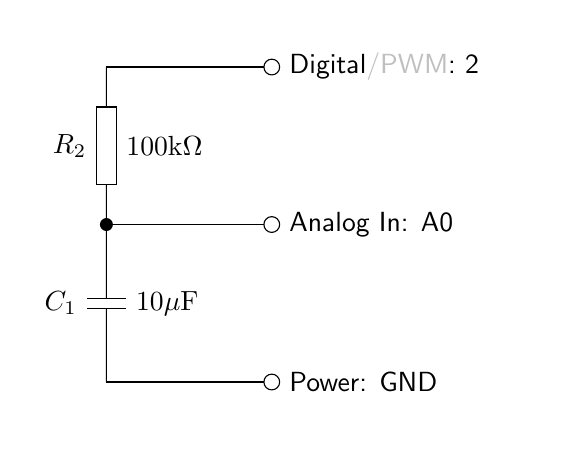
\begin{tikzpicture}[circuit ee IEC]
        % Background
        \draw[draw=none,fill=white] (1,0.5) rectangle ++(6.5,5);

        % Labels
        \node[anchor=west,font=\sffamily] at (4.2,5) {Digital\textcolor{gray!50}{/PWM}: 2};
        \node[anchor=west,font=\sffamily] at (4.2,3) {Analog In: A0};
        \node[anchor=west,font=\sffamily] at (4.2,1) {Power: GND};
        
        % Components
        \draw (2,5) to [resistor={info'=$R_{2}$,ohm=100k}] (2,3);
        \draw (2,3) to [capacitor={farad=10\mu,info'=$C_{1}$}] (2,1);

        % Circuit
        \draw[fill=black] (2,3) circle(0.75mm);
        \foreach \y in {1,3,5} {
            \draw (4.1,\y) circle(1mm);
            \draw (4,\y) -- ++(-2,0);
        }

    \end{tikzpicture}
\end{document}    